\chapter{基于属性解耦双模态提示的未见细胞核实例分割}

\section{研究背景与问题提出}
细胞核实例分割是数字病理分析中的基础问题，也是后续肿瘤分级、免疫微环境量化、空间组织学分析和疗效评估的关键前提。与普通前景分割相比，实例分割不仅需要识别哪些像素属于细胞核，还要进一步把相邻、接触甚至部分重叠的细胞核拆分为独立个体。病理图像中的细胞核密集、尺度变化大、染色风格复杂，因此这一问题长期依赖昂贵而细致的人工标注。

随着视觉语言预训练模型在开放词汇检测与分割任务中的成功，研究者开始尝试把文本提示引入医学图像分析。然而，与自然图像不同，病理图像中的类别描述高度细粒度，不同细胞亚型往往只在边缘清晰度、核形态、染色深浅和局部纹理上存在细微差异。单纯依赖类别名或者简单属性短语，难以让模型稳定区分未见类别和跨域场景中的复杂实例。因此，如何在不增加大量目标域标注的前提下，把文本提示和图像提示有机结合，并把支持图像中的关键结构信息转化为模型可用的提示信号，成为本章工作的核心问题。

本章对应作者发表于 IEEE Transactions on Medical Imaging 的工作 \emph{Dual-modal Vision-Language Prompting for Unseen Nuclei Instance Segmentation via Attribute Disentanglement}。该工作试图回答两个相互关联的问题：其一，未见类别的核实例分割能否仅依靠少量提示示例完成；其二，图像提示内部的不同结构成分是否应该被解耦建模，而不是简单压缩为单个全局向量。围绕这两个问题，本章提出属性解耦双模态提示框架，在统一视觉语言分割框架内显式建模文本提示、前景提示、轮廓提示和中心提示，从而增强模型对未见类别与跨域形态变化的适应能力。

\section{任务定义与形式化描述}
设源域训练集为
\[
\mathcal{D}_{\text{train}}=\{(x_i, y_i)\}_{i=1}^{N},
\]
其中 $x_i$ 表示病理图像块，$y_i$ 表示实例级细胞核标注。测试阶段面对的是未见目标域 $\mathcal{D}_{\text{test}}$，目标域不提供大规模像素级微调监督，只允许给出少量支持图像
\[\mathcal{S}=\{(s_j, a_j)\}_{j=1}^{K},
\]
其中 $s_j$ 为支持图像，$a_j$ 为与该图像相关的属性提示或由图像中前景、边缘、中心区域提取出的提示信息。模型需要基于源域学得的通用表示以及支持集提示，在查询图像 $q$ 上输出实例分割结果
\[
f(q \mid \mathcal{S}) = \{m_1,m_2,\dots,m_T\}.
\]

与传统 few-shot segmentation 不同，本章问题不是针对封闭类别在单一数据集内做支持--查询匹配，而是要在视觉语言预训练基础上，实现未见核类别与跨域核形态的统一适配。换言之，模型既要保留源域预训练得到的通用核结构认知，又要借助支持图像中细粒度的视觉先验快速补充目标域特征。因此，本章工作的关键不在于重新设计一个庞大的 few-shot 网络，而在于在原有视觉语言模型中构建一种低成本、结构清晰、可解释的双模态提示机制。

\section{研究动机}
文本提示能够提供抽象类别语义，但往往难以完整描述医学目标的局部形态差异。举例来说，“epithelial nucleus”和“neutrophil nucleus”虽然都可以用语言区分，但真实判别往往依赖细胞核大小、轮廓规则性、染色均匀程度以及与背景组织的关系。这些信息通过文字可以表达，但代价是需要大量精心设计的 prompt engineering。与之对应，支持图像天然包含上述视觉细节，因此更适合作为目标域适配时的结构先验。

然而，如果直接把整张支持图像编码为单个提示向量，再注入视觉语言模型，常常会把前景、背景和噪声混合到一起，导致提示表示不稳定。病理图像中尤其如此：细胞核前景本身、核边缘变化和核中心稳定区域分别携带不同的判别信息。前景区域负责表达主体形态，边缘区域负责实例分离和轮廓约束，中心区域则与核密集场景中的实例完整性和定位稳定性密切相关。基于这一观察，本章引入属性解耦思想，将视觉提示拆解为多个可解释分支，再把它们映射到统一的语言提示空间中。

\section{方法总体框架}
本章方法可以概括为“文本提示 + 图像提示 + 属性解耦 + 统一映射”四个步骤。首先，模型保留文本提示分支，用于提供高层类别语义和任务上下文；其次，从支持图像中分别抽取前景、边缘和中心三类结构性提示；再次，通过视觉文本化映射模块将这些提示变换到与语言 token 兼容的表示空间；最后，在解码和推理阶段联合使用多分支提示，以提升目标域未见核实例分割性能。

\begin{figure}[H]
  \centering
  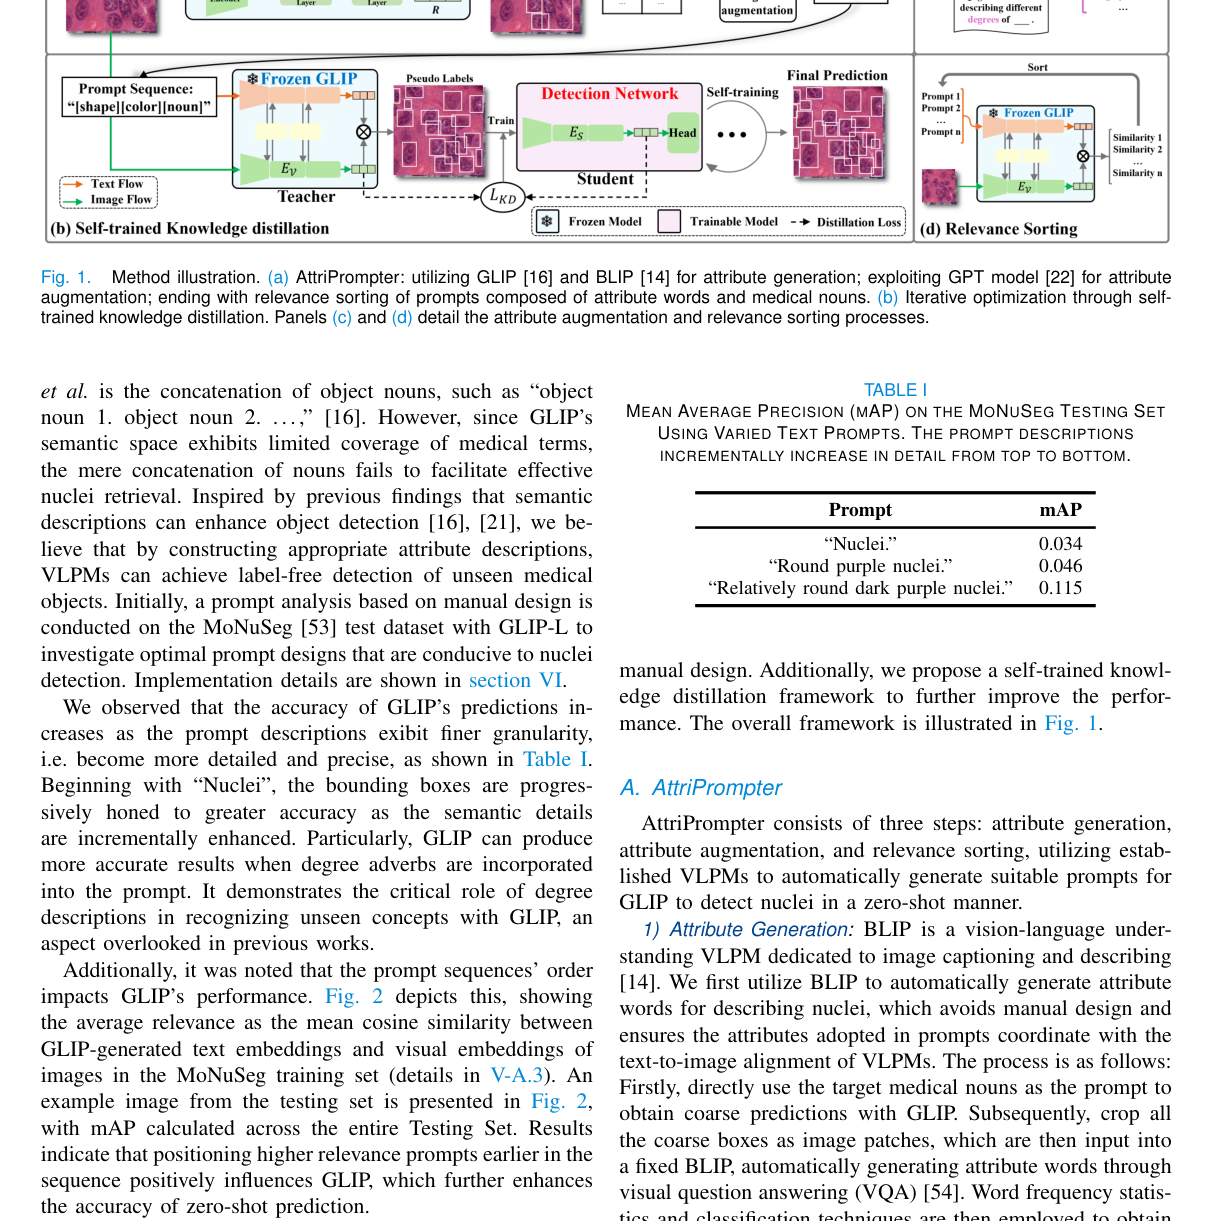
\includegraphics[width=\textwidth]{figures/tmi_fig_method.png}
  \caption{TMI 工作整体框架示意图。该图展示了文本提示分支与图像提示分支在统一视觉语言分割模型中的协同方式，其中图像提示进一步被解耦为前景、轮廓与中心三个子分支。}
  \label{fig:tmi_method}
\end{figure}

图 \ref{fig:tmi_method} 体现了本章方法的核心结构。与传统单一提示方案相比，该框架并未把所有支持信息压缩为一个粗糙的嵌入，而是强调不同结构提示在功能上的分工。文本分支回答“目标是什么”，前景分支强调“目标主体在哪里”，边缘分支回答“相邻目标如何分离”，中心分支则进一步稳定实例内部表示。通过这种方式，模型在未见类别和跨数据集迁移中获得更好的提示适配能力。

\section{属性解耦提示设计}
\subsection{文本提示分支}
文本提示分支负责提供类别语义与任务上下文，是整个框架中与视觉语言预训练最直接对齐的部分。与只使用单个类别名称相比，本章工作通过更丰富的属性描述，使文本提示不仅承担“命名”功能，还承担“引导模型聚焦关键形态”的功能。由于文本提示本身已经在源域训练中学习了语言到视觉的粗对齐，因此在测试阶段仍然是最稳定的高层先验来源。

\subsection{前景提示分支}
前景提示分支从支持图像中提取主体区域信息，其核心作用是帮助模型快速聚焦目标的主要形状和染色分布。该分支对跨域场景尤为重要，因为即使类别不变，不同医院、扫描仪和染色方案也会引入明显的风格差异。前景提示通过少量支持样本把这种目标域风格编码进提示空间，从而降低模型对源域统计的过度依赖。

\subsection{边缘提示分支}
边缘提示分支主要为实例分离服务。病理图像中的常见失败模式并不是完全漏检，而是多个相邻细胞核被错误粘连为一个大实例。因此，边缘信息往往比简单的前景分布更能决定实例分割质量。本章将轮廓提示显式作为独立分支建模，有利于让模型形成更强的边界敏感性。

\subsection{中心提示分支}
中心提示分支关注目标内部较稳定区域及其空间集中趋势，对密集核实例场景下的定位稳定性和目标独立性有辅助作用。它与边缘分支形成互补：边缘分支提供分离线索，中心分支提供内部一致性线索，两者共同帮助模型完成复杂密集场景中的实例拆分。

\section{视觉文本化映射模块}
视觉提示与文本提示原本位于不同表示空间，若直接拼接，往往会造成分布不一致和优化不稳定。因此，本章通过轻量的映射模块将视觉提示变换到与语言 token 兼容的空间中。这里的关键思想并不是“让图像替代文本”，而是“让图像成为另一种可与文本并列的提示表示”。

从工程实现上看，这一映射模块承担了两个作用。第一，它为不同结构分支提供统一接口，使前景、边缘和中心提示可以在同一语义空间中被组合。第二，它保留了原始视觉语言模型的主体结构，避免因大幅修改 backbone 或解码器而破坏预训练模型的稳定性。也正因为这一点，本章方法在少量目标域提示条件下就能快速工作，而不依赖昂贵的大规模目标域微调。

\section{训练策略与推理流程}
训练阶段，模型在源域上学习文本提示与视觉提示的联合使用方式，同时让映射模块和分支融合模块逐渐适应核实例分割任务。由于源域训练具有完整实例监督，模型能够在这一阶段学会如何把不同提示分支映射到分割判据上。测试阶段，不需要再进行大规模目标域微调，只需从目标域中选取少量支持样本，构造对应的文本与图像提示，即可在查询图像上进行实例分割。

这一训练--测试设计使本章方法同时兼顾了公平性和可迁移性。一方面，它保留了源域完整监督带来的稳定表示学习；另一方面，它又通过少量支持样本完成目标域适配，从而避免把大规模目标域标注和长时间微调作为前提条件。对于实际病理应用而言，这种“源域学习 + 目标域轻量提示”的范式更符合医学数据可获得性的现实。

\section{实验设计}
\subsection{跨域评测设置}
本章的核心实验围绕跨域核实例分割展开，典型任务包括 MoNuSAC$\rightarrow$CoNSeP、CoNSeP$\rightarrow$MoNuSAC 以及若干更具风格差异的跨域组合。评价指标使用 Dice、Hausdorff Distance、AJI、对象级 Dice、PQ 与 F1 等，既关注整体前景质量，也关注实例级分离能力。与只报告单个指标的做法相比，这样的评价体系更能全面反映分割器在复杂病理场景中的实际表现。

\subsection{消融实验设置}
为了验证属性解耦提示的必要性，本章特别设计了多组消融实验。其核心问题包括：只使用文本提示时性能如何；加入前景提示是否有显著增益；边缘和中心分支能否进一步改善粘连目标的分离质量；不同提示分支组合之间是否存在互补关系。这些问题共同构成了本章实验逻辑的主线。

\begin{figure}[H]
  \centering
  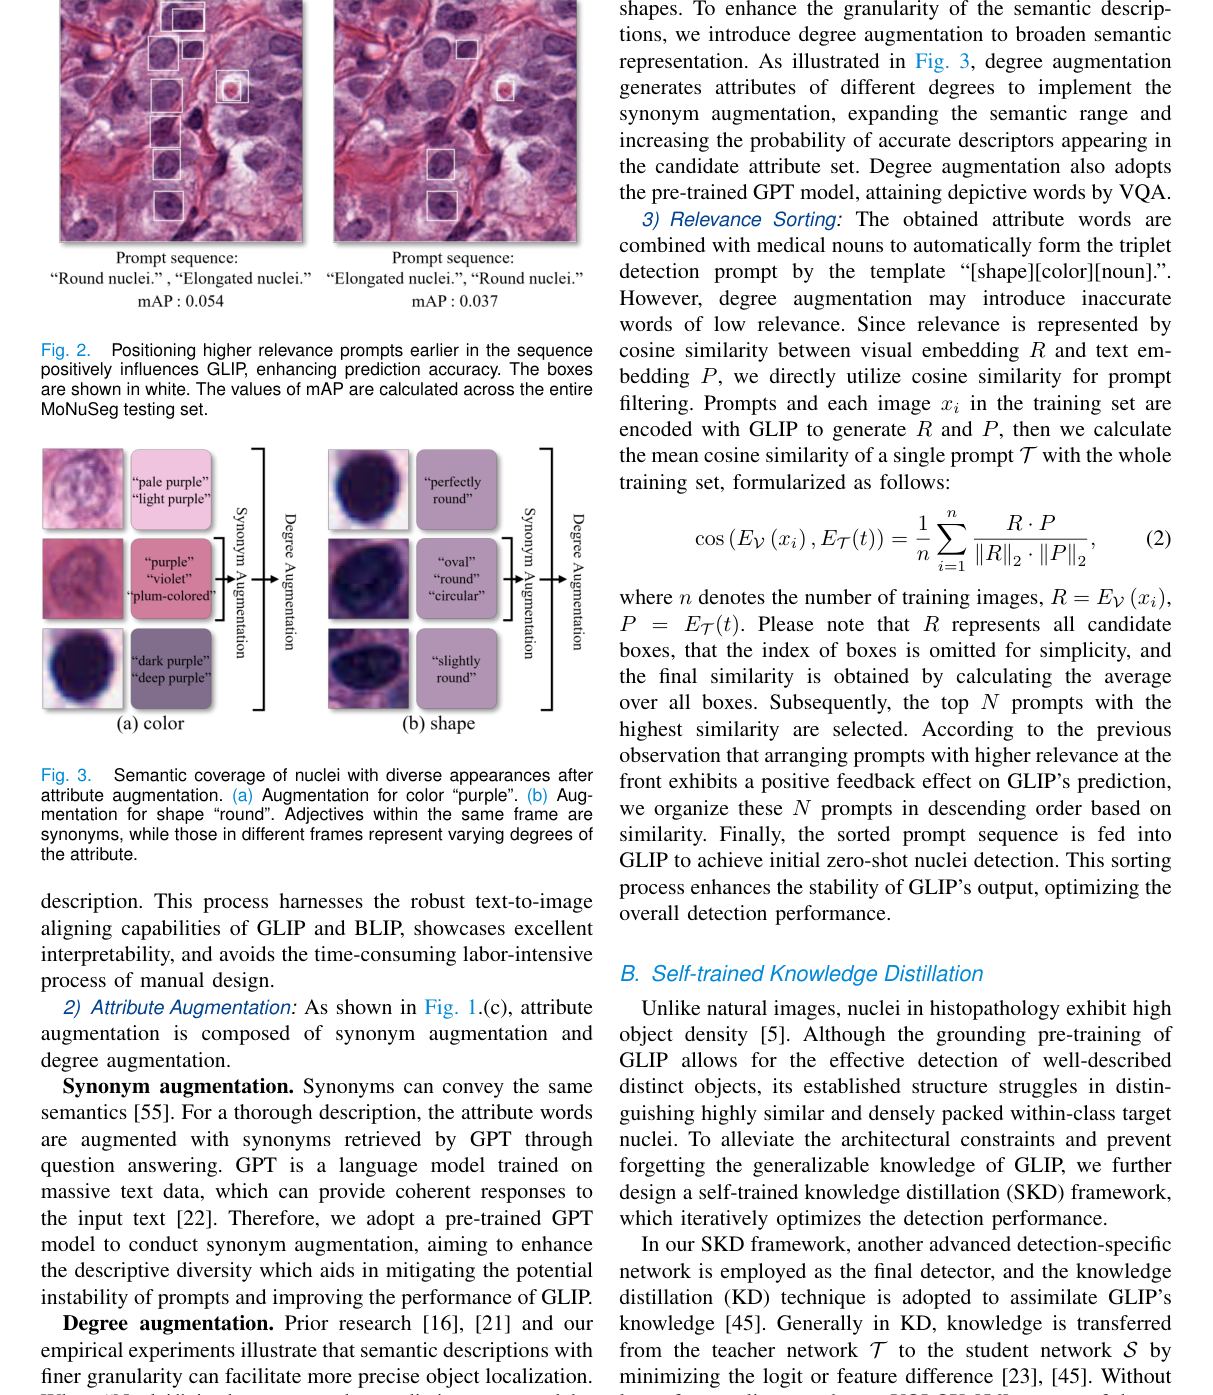
\includegraphics[width=\textwidth]{figures/tmi_fig_results.png}
  \caption{TMI 工作主要定性结果展示。不同提示策略在未见细胞核实例分割任务中呈现出明显差异，其中属性解耦提示在边界完整性、密集区域分离和目标一致性方面更具优势。}
  \label{fig:tmi_results}
\end{figure}

图 \ref{fig:tmi_results} 展示了典型的可视化结果。从这些结果可以直观看出，单一文本提示往往只能提供粗粒度前景，而加入图像提示后，模型更容易恢复细胞核真实边界；进一步使用属性解耦分支后，多个接触核之间的分离也更加清晰。这类定性结果与后续定量结果相互印证，说明本章方法并非仅在某个指标上投机取巧，而是在整体实例结构恢复上获得了更加一致的改进。

\begin{table}[H]
  \centering
  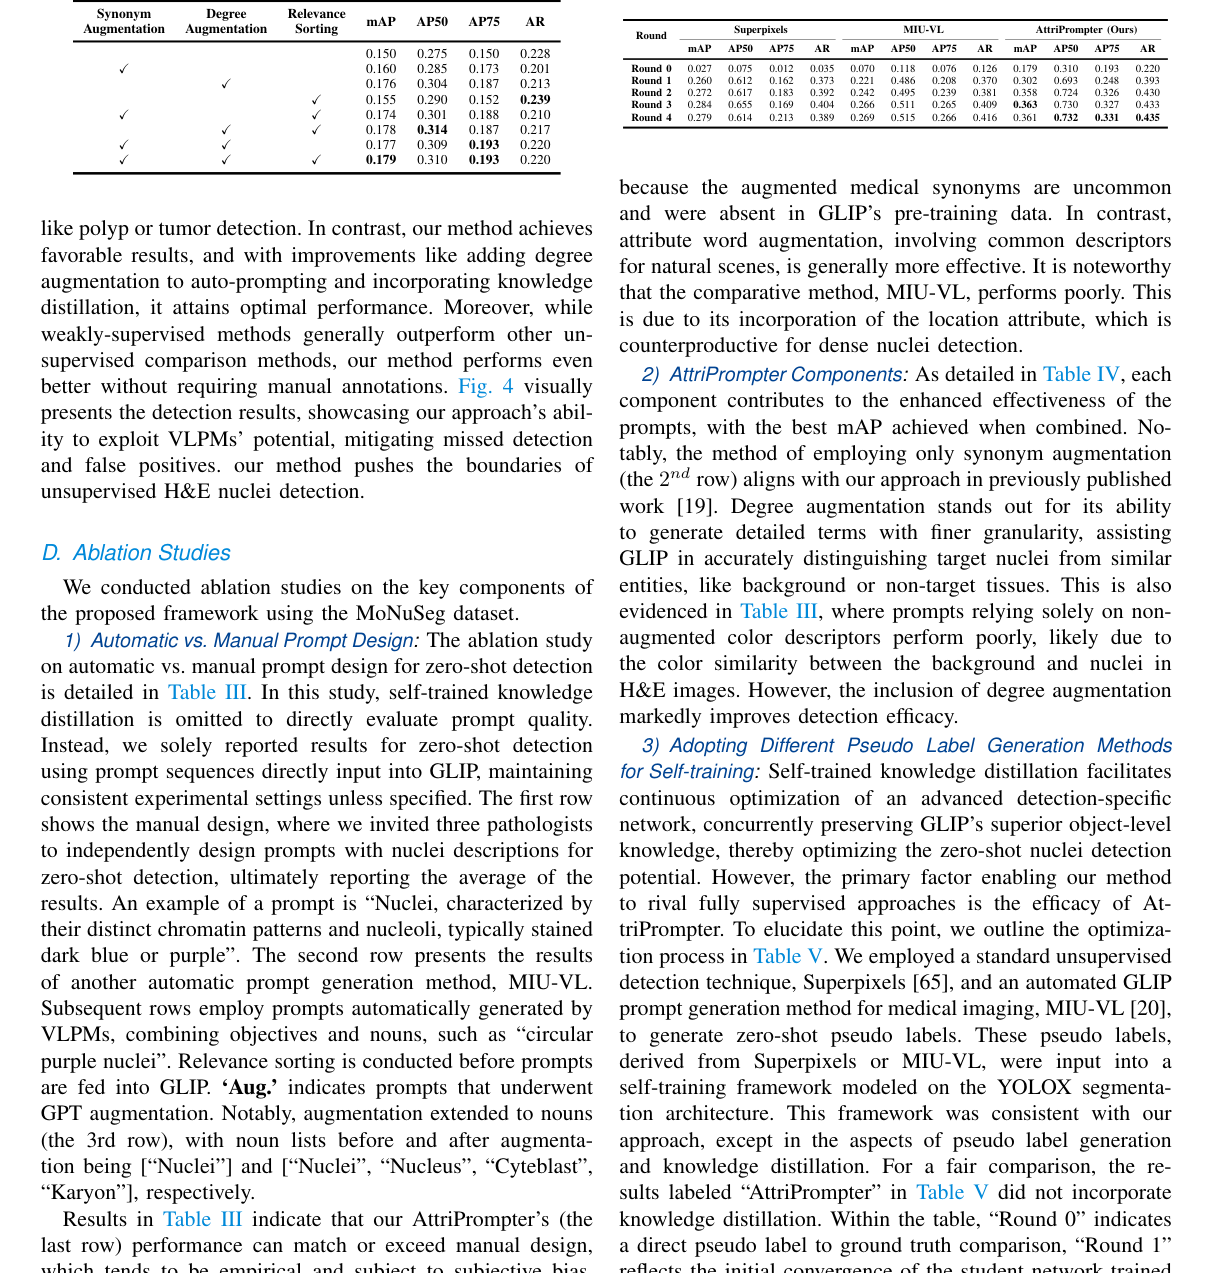
\includegraphics[width=\textwidth]{figures/tmi_table_ablation.png}
  \caption{TMI 工作的核心消融实验表。该表重点比较不同提示分支组合对检测指标与分割指标的影响，验证文本提示与图像提示的互补关系。}
  \label{tab:tmi_ablation}
\end{table}

\begin{table}[H]
  \centering
  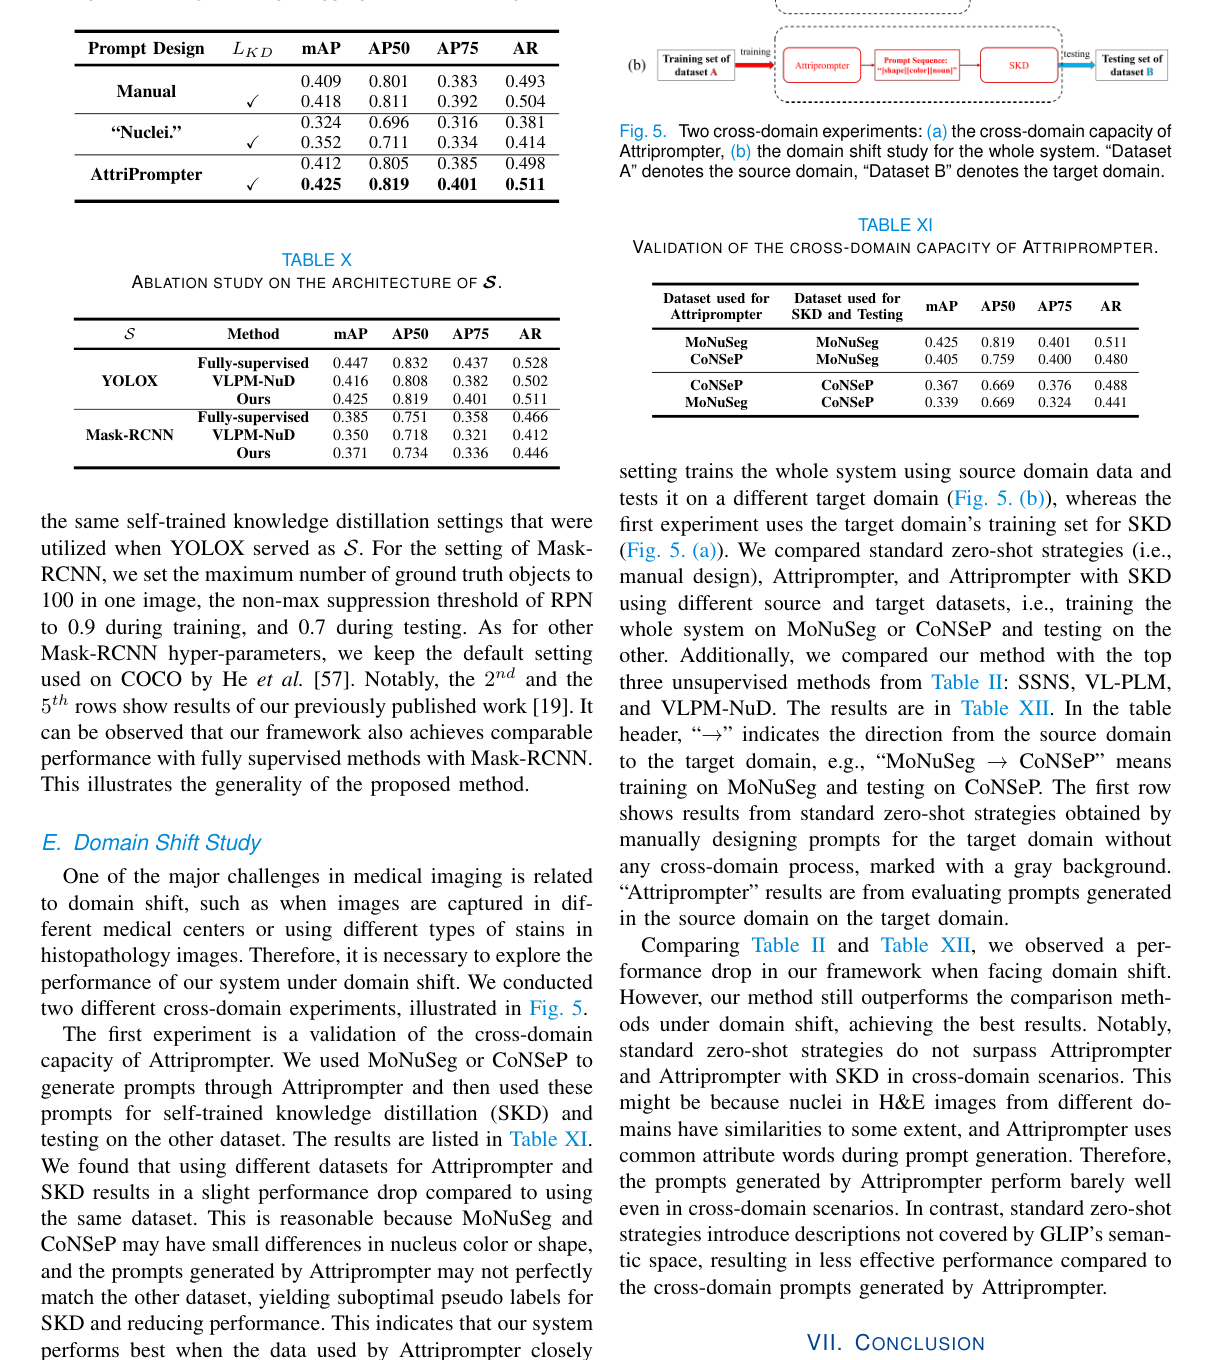
\includegraphics[width=\textwidth]{figures/tmi_table_more_ablation.png}
  \caption{TMI 工作的补充消融实验表。该表进一步分析属性提示解耦、不同映射方式及多分支融合策略对模型性能的影响。}
  \label{tab:tmi_more_ablation}
\end{table}

表 \ref{tab:tmi_ablation} 与表 \ref{tab:tmi_more_ablation} 共同构成了本章最重要的证据链。首先，文本提示是建立类别语义的基础，但若只保留文本，模型对细粒度结构差异的感知仍然不足。其次，前景、边缘和中心分支并不是简单重复信息，而是分别承担不同结构约束角色。当三个分支被联合使用时，模型通常能够在 Dice、AJI 和 PQ 等指标上取得更好的平衡。最后，映射方式与分支融合策略并不是中性的实现细节，而会直接影响提示是否能够稳定发挥作用。

\section{实验结果与讨论}
从定量结果看，本章方法在多个跨域核实例分割任务中都优于只依赖文本提示的基线模型，并且在若干场景下也优于只使用全局图像提示而不做属性解耦的方案。这说明图像提示并非越强越好，关键在于如何把提示内部的信息组织成模型真正能利用的结构化先验。属性解耦的价值，正体现在它把原本混杂的视觉信息拆解成若干可解释、可组合、可替换的提示元素。

从定性角度看，本章方法的改进尤其体现在三类场景。第一类是密集核实例区域，模型在加入边缘与中心提示后更容易把相邻目标分开；第二类是风格变化较大的跨域图像，前景提示能够帮助模型快速适配目标域染色差异；第三类是未见类别或形态变化明显的细胞类型，此时文本分支和视觉分支的联合提示能够提供更丰富的判别依据。换言之，本章方法的优势并不局限于某一单一场景，而是体现在不同类型困难样本上的整体稳健性。

\section{局限性分析}
尽管本章方法在未见核实例分割中表现出较强潜力，但仍存在若干局限。首先，图像提示仍然依赖支持样本的代表性，若目标域支持图像本身质量较差或覆盖不足，性能提升可能受到限制。其次，多分支提示虽然带来更强的结构表达，但也增加了系统复杂度，需要在提示质量与推理效率之间进行权衡。再次，本章仍然主要基于二维病理 patch 进行实验，未来若扩展到更大视野甚至全切片场景，提示构造与融合方式可能仍需进一步调整。

\section{本章创新点总结}
本章的主要创新可以归纳为四点。第一，将未见类别核实例分割问题统一到视觉语言提示学习框架中，使文本提示与图像提示在同一模型内协同工作。第二，提出属性解耦提示机制，把图像提示拆解为前景、边缘和中心三个结构性分支，增强模型对细粒度实例结构的表达能力。第三，设计视觉文本化映射模块，使视觉提示能够与语言 token 在统一空间中融合，从而兼容已有视觉语言模型主体结构。第四，通过系统性的跨域实验与消融分析，验证了多分支提示在未见类别和跨域核实例分割中的有效性。

\section{与全文主线的关系}
如果说第二章和第三章之前的相关工作主要奠定了视觉语言模型与弱监督/零样本医学视觉任务的背景，那么本章可以视为全文的中心工作之一。它不仅把文本提示从“类别名描述”推进到“结构化语义提示”，也把图像示例从“支持图像”推进到“可映射为语言空间的提示表示”。这一思想直接影响后续第五章的 VisTex 工作，也为后续基于支持图像的直接测试和跨域适配实验提供了概念基础。

\section{本章小结}
本章围绕未见细胞核实例分割问题，系统介绍了基于属性解耦双模态提示的解决思路。通过文本提示、前景提示、边缘提示和中心提示的联合建模，模型能够在保持视觉语言预训练优势的同时，更充分利用少量支持图像中的结构信息。实验结果表明，该方法能够在多个跨域实例分割任务中获得稳定收益，并为后续图像提示检测与更复杂数字病理分析任务奠定了坚实基础。
